\newpage
\subsubsection{Flight Report: Mount Stability}
\begin{minipage}{1\textwidth}
	\begin{flushright}
		Date: 29-05-2022\\
		Location: Near Sunrise Riverside Block K\\
		Coordinates: 10.724144, 106.704113\\
		Flight Mode: \gls{GPS}\\
		Flight Duration: 15 minutes\\\vspace{5mm}
	\end{flushright}
\end{minipage}

The goal of this flight was to check if the drone was stable when flying with the second revision of the sensor package as described in the Design Report. \cite{designreport}

\begin{figure}[h]
\centering
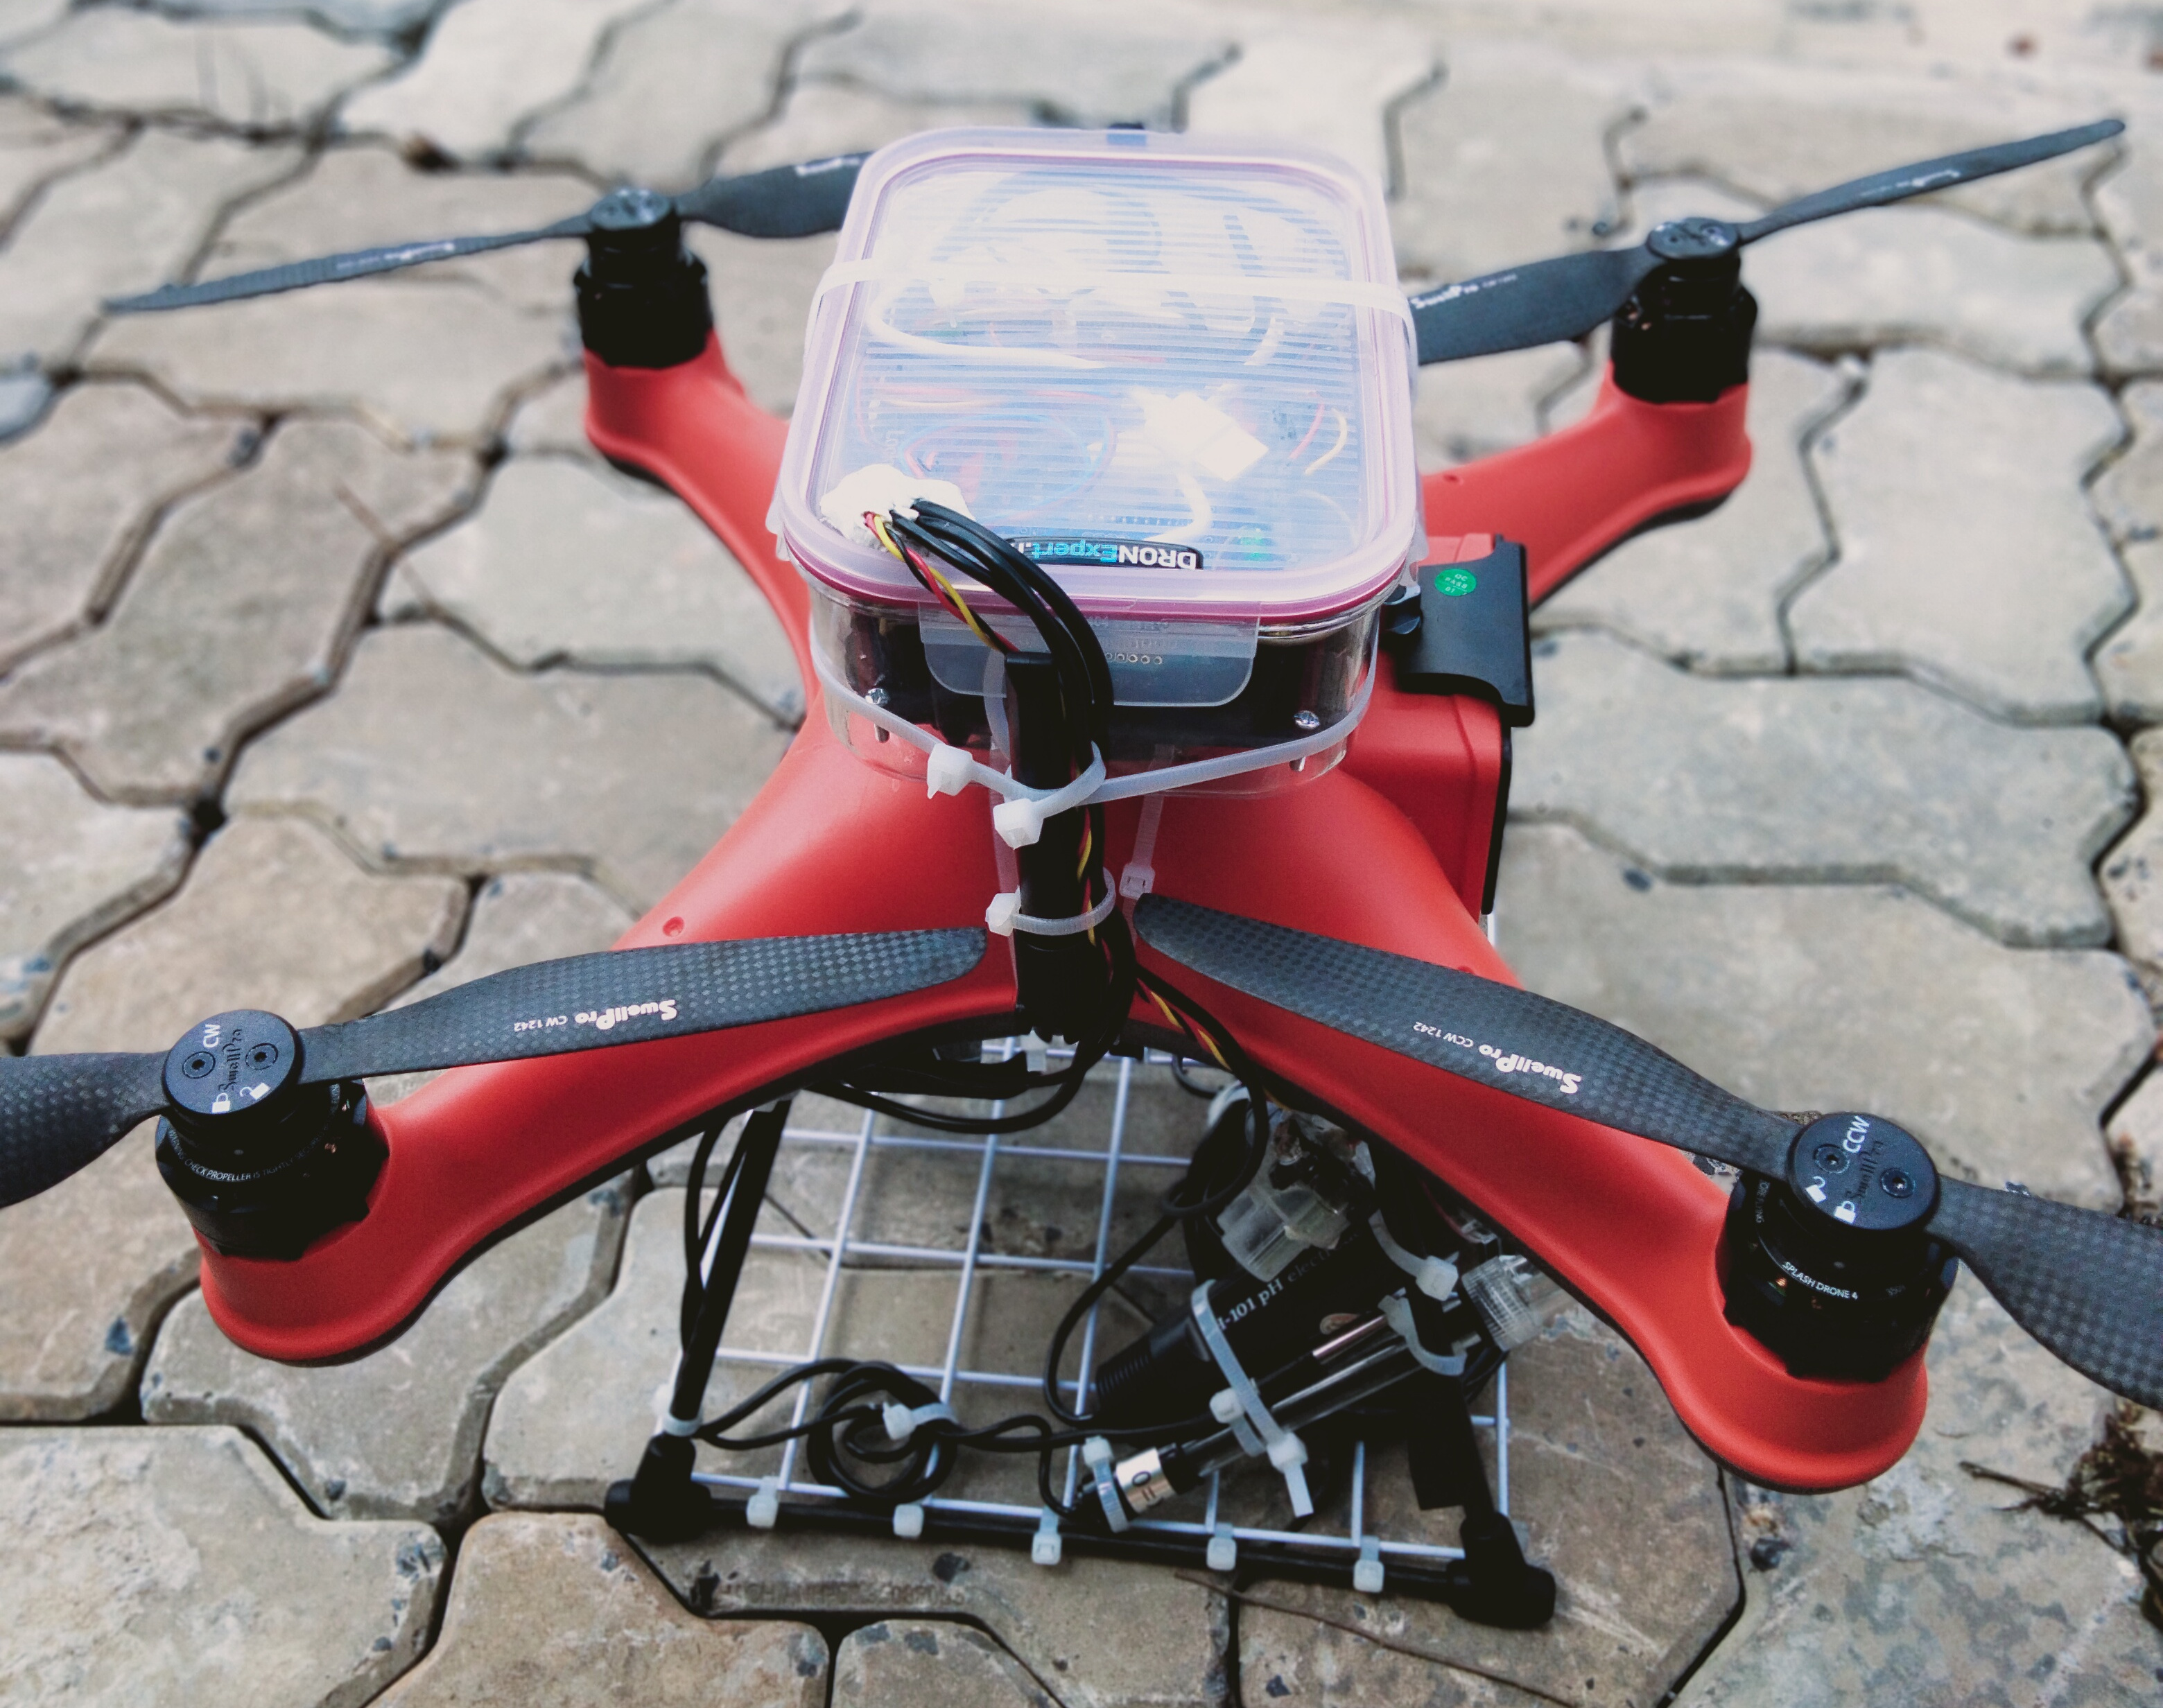
\includegraphics[scale=0.4]{080_testing/flights/21_drone.jpg}
\caption{Drone with the second revision of the sensor package [own picture]}
\end{figure}

The drone flew for 15 minutes around a grass field at different speeds and altitudes. In the following sections, potential risks will be elaborated and evaluated based on this test flight.

\paragraph{The center of mass could be shifted too much}
Due to the sensor placement on the bottom of the drone, the center of mass could be shifted too much, causing drift to one direction. During this test flight, I did not experience such a thing. The drone did not drift to any direction during the whole flight.\\

While changing directions, I did notice the drone took some more space and time to stabilize its position.

\paragraph{The drone could be too heavy}
Due to the weight of the sensor package, the drone might not be able to take off or remain a stable altitude during flight. During this test flight, I noticed that the drone took far more force to take off. The drone needed manual assistance with the remote control to remain the same altitude.

\paragraph{The sensor package could not be stable enough}
Due to the mounting solution, the electronics enclosure and the sensors could move or fall off during flight. During this test flight, this did not happen. The enclosure and sensors were not moving

\paragraph{The sensor is blocking the view of the camera}
Due to the mounting solution, the electronics enclosure and the sensors could move or fall off during flight. During this test flight, this did not happen. The enclosure and sensors seemed stable, even when moving the drone at fast speeds

\paragraph{The electronics enclosure could block the propellers}
The electronics enclosure could not make it possible for the propellers move freely during flight, this could result in a crash. During this test flight, this did not happen. There was ample space for the propellers to move freely, even when moving the drone at fast speeds

\paragraph{Conclusion}
While manual intervention is sometimes necessary, I feel comfortable enough to perform a full test flight in the water.